\PassOptionsToPackage{unicode=true}{hyperref} % options for packages loaded elsewhere
\PassOptionsToPackage{hyphens}{url}
%
\documentclass[a4paper,11pt]{memoir}
\usepackage{lmodern}
\usepackage{amssymb,amsmath}
\usepackage{ifxetex,ifluatex}
\usepackage{fixltx2e} % provides \textsubscript
\ifnum 0\ifxetex 1\fi\ifluatex 1\fi=0 % if pdftex
  \usepackage[T1]{fontenc}
  \usepackage[utf8]{inputenc}
  \usepackage{textcomp} % provides euro and other symbols
\else % if luatex or xelatex
  \usepackage{unicode-math}
  \defaultfontfeatures{Ligatures=TeX,Scale=MatchLowercase}
\fi
% use upquote if available, for straight quotes in verbatim environments
\IfFileExists{upquote.sty}{\usepackage{upquote}}{}
% use microtype if available
\IfFileExists{microtype.sty}{%
\usepackage[]{microtype}
\UseMicrotypeSet[protrusion]{basicmath} % disable protrusion for tt fonts
}{}
\IfFileExists{parskip.sty}{%
\usepackage{parskip}
}{% else
\setlength{\parindent}{0pt}
\setlength{\parskip}{6pt plus 2pt minus 1pt}
}
\usepackage{hyperref}
\hypersetup{
            pdftitle={Re-encoding people in the EDH dataset},
            pdfborder={0 0 0},
            breaklinks=true}
\urlstyle{same}  % don't use monospace font for urls
\usepackage[left=2cm,right=2cm,top=2cm,bottom=2cm]{geometry}
\usepackage{color}
\usepackage{fancyvrb}
\newcommand{\VerbBar}{|}
\newcommand{\VERB}{\Verb[commandchars=\\\{\}]}
\DefineVerbatimEnvironment{Highlighting}{Verbatim}{commandchars=\\\{\}}
% Add ',fontsize=\small' for more characters per line
\usepackage{framed}
\definecolor{shadecolor}{RGB}{248,248,248}
\newenvironment{Shaded}{\begin{snugshade}}{\end{snugshade}}
\newcommand{\AlertTok}[1]{\textcolor[rgb]{0.94,0.16,0.16}{#1}}
\newcommand{\AnnotationTok}[1]{\textcolor[rgb]{0.56,0.35,0.01}{\textbf{\textit{#1}}}}
\newcommand{\AttributeTok}[1]{\textcolor[rgb]{0.77,0.63,0.00}{#1}}
\newcommand{\BaseNTok}[1]{\textcolor[rgb]{0.00,0.00,0.81}{#1}}
\newcommand{\BuiltInTok}[1]{#1}
\newcommand{\CharTok}[1]{\textcolor[rgb]{0.31,0.60,0.02}{#1}}
\newcommand{\CommentTok}[1]{\textcolor[rgb]{0.56,0.35,0.01}{\textit{#1}}}
\newcommand{\CommentVarTok}[1]{\textcolor[rgb]{0.56,0.35,0.01}{\textbf{\textit{#1}}}}
\newcommand{\ConstantTok}[1]{\textcolor[rgb]{0.00,0.00,0.00}{#1}}
\newcommand{\ControlFlowTok}[1]{\textcolor[rgb]{0.13,0.29,0.53}{\textbf{#1}}}
\newcommand{\DataTypeTok}[1]{\textcolor[rgb]{0.13,0.29,0.53}{#1}}
\newcommand{\DecValTok}[1]{\textcolor[rgb]{0.00,0.00,0.81}{#1}}
\newcommand{\DocumentationTok}[1]{\textcolor[rgb]{0.56,0.35,0.01}{\textbf{\textit{#1}}}}
\newcommand{\ErrorTok}[1]{\textcolor[rgb]{0.64,0.00,0.00}{\textbf{#1}}}
\newcommand{\ExtensionTok}[1]{#1}
\newcommand{\FloatTok}[1]{\textcolor[rgb]{0.00,0.00,0.81}{#1}}
\newcommand{\FunctionTok}[1]{\textcolor[rgb]{0.00,0.00,0.00}{#1}}
\newcommand{\ImportTok}[1]{#1}
\newcommand{\InformationTok}[1]{\textcolor[rgb]{0.56,0.35,0.01}{\textbf{\textit{#1}}}}
\newcommand{\KeywordTok}[1]{\textcolor[rgb]{0.13,0.29,0.53}{\textbf{#1}}}
\newcommand{\NormalTok}[1]{#1}
\newcommand{\OperatorTok}[1]{\textcolor[rgb]{0.81,0.36,0.00}{\textbf{#1}}}
\newcommand{\OtherTok}[1]{\textcolor[rgb]{0.56,0.35,0.01}{#1}}
\newcommand{\PreprocessorTok}[1]{\textcolor[rgb]{0.56,0.35,0.01}{\textit{#1}}}
\newcommand{\RegionMarkerTok}[1]{#1}
\newcommand{\SpecialCharTok}[1]{\textcolor[rgb]{0.00,0.00,0.00}{#1}}
\newcommand{\SpecialStringTok}[1]{\textcolor[rgb]{0.31,0.60,0.02}{#1}}
\newcommand{\StringTok}[1]{\textcolor[rgb]{0.31,0.60,0.02}{#1}}
\newcommand{\VariableTok}[1]{\textcolor[rgb]{0.00,0.00,0.00}{#1}}
\newcommand{\VerbatimStringTok}[1]{\textcolor[rgb]{0.31,0.60,0.02}{#1}}
\newcommand{\WarningTok}[1]{\textcolor[rgb]{0.56,0.35,0.01}{\textbf{\textit{#1}}}}
\usepackage{graphicx,grffile}
\makeatletter
\def\maxwidth{\ifdim\Gin@nat@width>\linewidth\linewidth\else\Gin@nat@width\fi}
\def\maxheight{\ifdim\Gin@nat@height>\textheight\textheight\else\Gin@nat@height\fi}
\makeatother
% Scale images if necessary, so that they will not overflow the page
% margins by default, and it is still possible to overwrite the defaults
% using explicit options in \includegraphics[width, height, ...]{}
\setkeys{Gin}{width=\maxwidth,height=\maxheight,keepaspectratio}
\setlength{\emergencystretch}{3em}  % prevent overfull lines
\providecommand{\tightlist}{%
  \setlength{\itemsep}{0pt}\setlength{\parskip}{0pt}}
\setcounter{secnumdepth}{0}
% Redefines (sub)paragraphs to behave more like sections
\ifx\paragraph\undefined\else
\let\oldparagraph\paragraph
\renewcommand{\paragraph}[1]{\oldparagraph{#1}\mbox{}}
\fi
\ifx\subparagraph\undefined\else
\let\oldsubparagraph\subparagraph
\renewcommand{\subparagraph}[1]{\oldsubparagraph{#1}\mbox{}}
\fi

% set default figure placement to htbp
\makeatletter
\def\fps@figure{htbp}
\makeatother

\usepackage{hyperref}
\PassOptionsToPackage{bookmarks=false}{hyperref}
\setmainfont{Tempora}
\usepackage{polyglossia}
\setdefaultlanguage{english}
\setotherlanguage[variant=ancient]{greek}

\makeatletter
\renewcommand{\figurename}{Fig.}
\renewcommand{\thefigure}{\@arabic\c@figure}
\makeatother

\setcounter{page}{9}
\setcounter{figure}{1}

\title{Re-encoding \texttt{people} in the \texttt{EDH} dataset}
\author{Antonio Rivero Ostoic}
\date{September 2022}

\begin{document}
\maketitle

%   \hypertarget{preliminaries}{%
%   \subsection{Preliminaries}\label{preliminaries}}
%   
%   Install and load a version of \texttt{"sdam"} package.
%   
%   \begin{Shaded}
%   \begin{Highlighting}[]
%   \KeywordTok{install.packages}\NormalTok{(}\StringTok{"sdam"}\NormalTok{) }\CommentTok{# from CRAN}
%   \NormalTok{devtools}\OperatorTok{::}\KeywordTok{install_github}\NormalTok{(}\StringTok{"sdam-au/sdam"}\NormalTok{) }\CommentTok{# development version}
%   \NormalTok{devtools}\OperatorTok{::}\KeywordTok{install_github}\NormalTok{(}\StringTok{"mplex/cedhar"}\NormalTok{, }\DataTypeTok{subdir=}\StringTok{"pkg/sdam"}\NormalTok{) }\CommentTok{# legacy version R 3.6.x}
%   \end{Highlighting}
%   \end{Shaded}

\begin{Shaded}
\begin{Highlighting}[]
\CommentTok{# load and check versions}
\KeywordTok{library}\NormalTok{(sdam)}
\KeywordTok{packageVersion}\NormalTok{(}\StringTok{"sdam"}\NormalTok{)}
\end{Highlighting}
\end{Shaded}

\begin{verbatim}
[1] '1.0.0'
\end{verbatim}

\hypertarget{edh-people}{%
\section{EDH people}\label{edh-people}}

\begin{itemize}
\tightlist
\item
  \texttt{EDH} is a dataset in \texttt{"sdam"} that contains the texts
  of Latin and Latin-Greek inscriptions of the Roman Empire, which have
  been retrieved from the
  \href{https://edh-www.adw.uni-heidelberg.de/data/api}{Epigraphic
  Database Heidelberg API repository} through routines
  \texttt{get.edh()} and \texttt{get.edhw()}.
\end{itemize}

Since the year 2022 and still today, the API repository does not support
people variables, and the \texttt{EDH} dataset serves as an alternative
for the analysis of people-related inscriptions.

One challenge with people variables in \texttt{EDH} is that some records
contain characters in Greek and Latin extended that need re-encoding for
a proper rendering and display.

\hypertarget{re-encoding-people-in-edh}{%
\subsection{\texorpdfstring{Re-encoding \texttt{people} in
\texttt{EDH}}{Re-encoding people in EDH}}\label{re-encoding-people-in-edh}}

Ancient inscriptions in some Roman provinces have Greek characters
written and, due to encoding and decoding steps in the process of
extraction, loading, and transformation of the data (perhaps Treating
UTF-8 Bytes as Windows-1252?), Greek and other Latin characters are not
displayed properly with the actual version of the \texttt{EDH} dataset.
Most of the encoding issues are in variables related to people, and some
examples with inscriptions in Roman provinces are next.

\hypertarget{achaia}{%
\subsubsection{Achaia}\label{achaia}}

The Roman province of \textbf{Achaia} in the \texttt{EDH} dataset has
inscriptions related to people.


\begin{figure}

{\centering 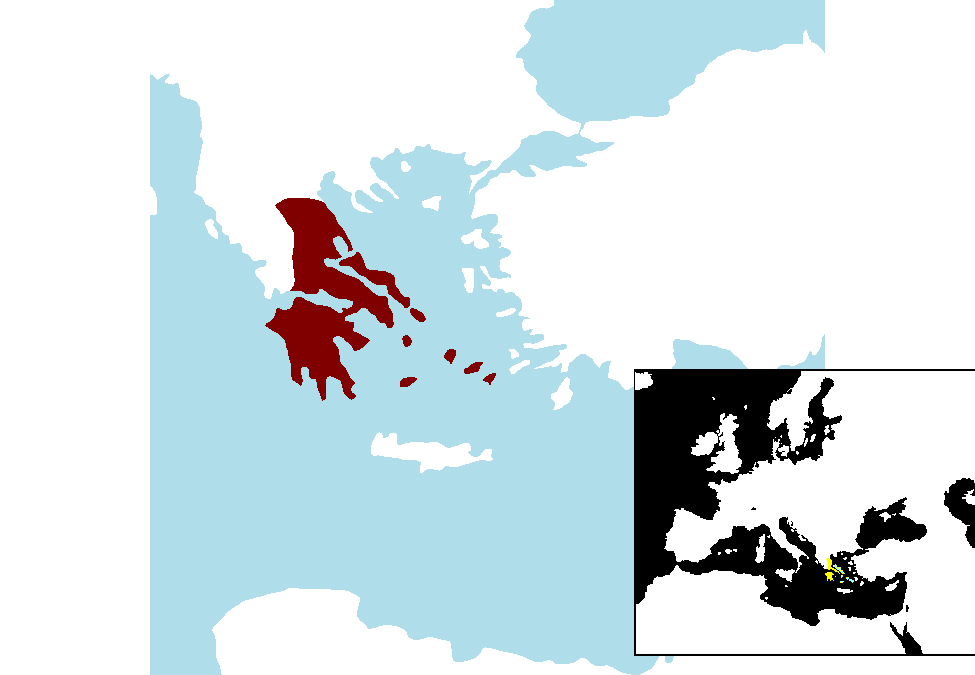
\includegraphics[width=0.25\linewidth]{img/unnamed-chunk-3-1} 

}

\caption{Roman province of Achaia (ca 117 AD).}\label{fig:unnamed-chunk-3}
\end{figure}

Function \texttt{edhw()} is to obtain the available inscriptions per
province in the EDH dataset, which is a list that is the input for the
same function to extract \texttt{people} variables \emph{cognomen} and
\emph{nomen}. In this case, the
\texttt{\textquotesingle{}province\textquotesingle{}} argument is
\texttt{Ach} that stands for \texttt{Achaia}.

\begin{Shaded}
\begin{Highlighting}[]
\CommentTok{# select two people variables from Achaia}
\NormalTok{Ach <-}\StringTok{ }\KeywordTok{edhw}\NormalTok{(}\DataTypeTok{province=}\StringTok{"Ach"}\NormalTok{) }\OperatorTok{|}\ErrorTok{>}\StringTok{ }
\StringTok{  }\KeywordTok{edhw}\NormalTok{(}\DataTypeTok{vars=}\StringTok{"people"}\NormalTok{, }\DataTypeTok{select=}\KeywordTok{c}\NormalTok{(}\StringTok{"cognomen"}\NormalTok{,}\StringTok{"nomen"}\NormalTok{))}
\end{Highlighting}
\end{Shaded}

There are 1539 records with people in \texttt{Ach} that corresponds to
the number of rows in this data frame.

\begin{Shaded}
\begin{Highlighting}[]
\CommentTok{# number of people entries in Achaia}
\KeywordTok{nrow}\NormalTok{(Ach)}
\end{Highlighting}
\end{Shaded}

\begin{verbatim}
[1] 1539
\end{verbatim}

However, some records have either missing data or are inscriptions where
\emph{cognomen} and \emph{nomen} are not available.

\begin{Shaded}
\begin{Highlighting}[]
\CommentTok{# also remove NAs}
\NormalTok{Ach <-}\StringTok{ }\KeywordTok{edhw}\NormalTok{(}\DataTypeTok{province=}\StringTok{"Ach"}\NormalTok{) }\OperatorTok{|}\ErrorTok{>}\StringTok{ }
\StringTok{  }\KeywordTok{edhw}\NormalTok{(}\DataTypeTok{vars=}\StringTok{"people"}\NormalTok{, }\DataTypeTok{select=}\KeywordTok{c}\NormalTok{(}\StringTok{"cognomen"}\NormalTok{,}\StringTok{"nomen"}\NormalTok{), }\DataTypeTok{na.rm=}\OtherTok{TRUE}\NormalTok{)}

\KeywordTok{nrow}\NormalTok{(Ach)}
\end{Highlighting}
\end{Shaded}

\begin{verbatim}
[1] 1465
\end{verbatim}

\hypertarget{clean-function-for-re-encoding}{%
\subsection{Clean function for
re-encoding}\label{clean-function-for-re-encoding}}

Treating with \texttt{people} attribute variables requires many times
re-encoding that is one option in function \texttt{cln()}. For instance,
values in \emph{cognomen} in the first entries of \texttt{Ach} are
likely in Greek.

\begin{Shaded}
\begin{Highlighting}[]
\CommentTok{# some people entries in Achaia}
\KeywordTok{head}\NormalTok{(Ach)}
\end{Highlighting}
\end{Shaded}

\begin{verbatim}
        id                                            cognomen                   nomen
1 HD001917                                               Rufus Ponponius (= Pomponius)
2 HD001917                                                 Eia   Ponponia (= Pomponia)
3 HD001917                          Î<U+0094>όξα Î\235ίκη                    <NA>
4 HD002097 Î<U+0092>αλλενÏ<U+0084>ινιανόÏ<U+0082>+                    <NA>
5 HD002097                           Î<U+0092>άληÏ<U+0082>                    <NA>
6 HD002097                                           Arcadius+                    <NA>
\end{verbatim}

Function \texttt{cln()} serves to re-encode Greek and Latin characters
to render Greek, Greek extended, and Latin extended glyphs.

\begin{Shaded}
\begin{Highlighting}[]
\CommentTok{# re-encode in Ach cognomen}
\NormalTok{Ach}\OperatorTok{$}\NormalTok{cognomen }\OperatorTok{|}\ErrorTok{>}\StringTok{ }
\StringTok{  }\KeywordTok{head}\NormalTok{() }\OperatorTok{|}\ErrorTok{>}\StringTok{ }
\StringTok{  }\KeywordTok{cln}\NormalTok{()}
\end{Highlighting}
\end{Shaded}

\begin{verbatim}
cognomen
\end{verbatim}

\noindent
Rufus \\
Eia \\
ΔόξαΝίκη \\
Βαλλεντινιανός+ \\
Βάλης \\
Arcadius+ \\

\bigbreak 

For \emph{cognomen} in the last people entries in \texttt{Achaia}.

\begin{Shaded}
\begin{Highlighting}[]
\CommentTok{# last entries}
\KeywordTok{tail}\NormalTok{(Ach)}
\end{Highlighting}
\end{Shaded}

\begin{verbatim}
           id                                                                       cognomen
1534 HD068263                                             Î<U+009A>άλλÏ<U+0085>Ï<U+0082>
1535 HD068315 ΦÏ\201ονÏ<U+0084>εá¿<U+0096>νοÏ<U+0082> Î\235εικήÏ\201αÏ<U+0084>οÏ<U+0082>
1536 HD068319 ΦÏ\201ονÏ<U+0084>εá¿<U+0096>νοÏ<U+0082> Î\235εικήÏ\201αÏ<U+0084>οÏ<U+0082>
1537 HD072342                                          Î<U+0091>ἰμιλιανόÏ<U+0082>+
1538 HD072342                                             Î<U+009A>αιλιανόÏ<U+0082>+
1539 HD078079                                                                          Eburo
                               nomen
1534                            <NA>
1535 Î<U+009A>λαύδιοÏ<U+0082>
1536 Î<U+009A>λαύδιοÏ<U+0082>
1537 Î<U+009F>á½\220á½±Ï\201ιοÏ<U+0082>+
1538                            <NA>
1539                            <NA>
\end{verbatim}

After re-encoding the last records in \texttt{Ach} with \texttt{cln()},
it is easier to see, for example, that some have identical
\emph{cognomen} where entries having
\texttt{\textless{}NA\textgreater{}} in the input become \texttt{NA}.

\begin{Shaded}
\begin{Highlighting}[]
\CommentTok{# clean last entries of cognomen}
\NormalTok{Ach}\OperatorTok{$}\NormalTok{cognomen }\OperatorTok{|}\ErrorTok{>}\StringTok{ }
\StringTok{  }\KeywordTok{tail}\NormalTok{() }\OperatorTok{|}\ErrorTok{>}\StringTok{ }
\StringTok{  }\KeywordTok{cln}\NormalTok{()}
\end{Highlighting}
\end{Shaded}

\begin{verbatim}
cognomen
\end{verbatim}

\noindent
Κάλλυς \\
ΦροντεῖνοςΝεικήρατος \\
ΦροντεῖνοςΝεικήρατος \\
Αἰμιλιανός+ \\
Καιλιανός+\\
Eburo\\

\begin{Shaded}
\begin{Highlighting}[]
\CommentTok{# clean last entries of nomen}
\NormalTok{Ach}\OperatorTok{$}\NormalTok{nomen }\OperatorTok{|}\ErrorTok{>}\StringTok{ }
\StringTok{  }\KeywordTok{tail}\NormalTok{() }\OperatorTok{|}\ErrorTok{>}\StringTok{ }
\StringTok{  }\KeywordTok{cln}\NormalTok{()}
\end{Highlighting}
\end{Shaded}

\begin{verbatim}
nomen
\end{verbatim}

\noindent
NA \\
Κλαύδιος \\
Κλαύδιος \\
Οὐάριος+ \\
NA \\
NA\\


\hypertarget{re-encode-greek-and-latin-within-data-frames}{%
\subsection{Re-encode Greek and Latin within data
frames}\label{re-encode-greek-and-latin-within-data-frames}}

\hypertarget{aegyptus}{%
\subsubsection{Aegyptus}\label{aegyptus}}

In the case of the province of \textbf{Aegyptus}, three people variables
have a mixing og Greek and Latin characters scripted that need
\emph{re-codification} as well.

\begin{figure}[!h]

{\centering 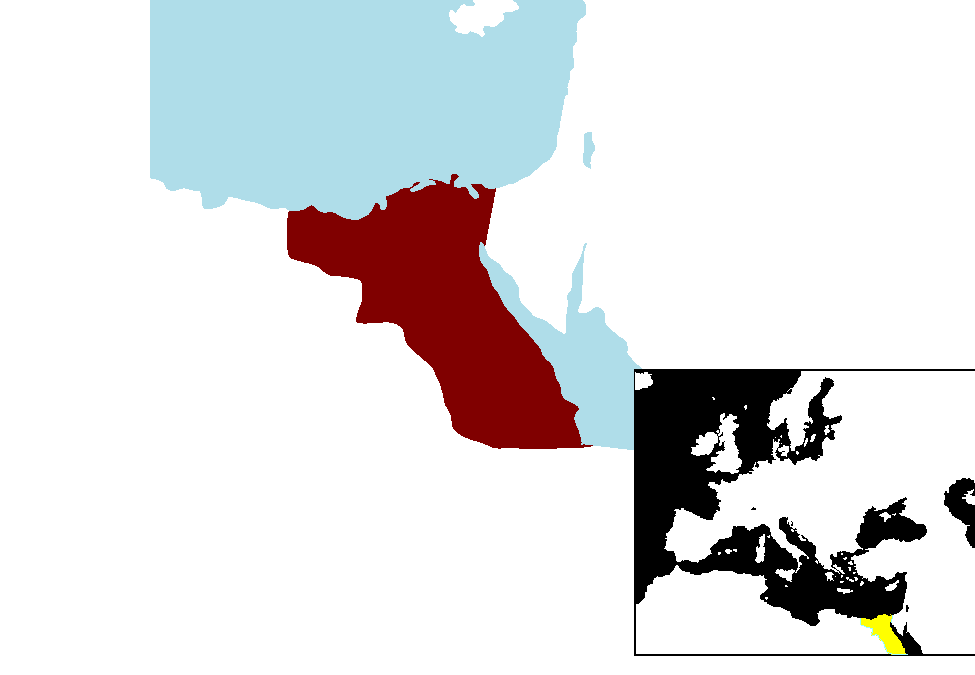
\includegraphics[width=0.25\linewidth]{img/unnamed-chunk-33-1} 

}

\caption{Roman province of Aegyptus (ca 117 AD).}\label{fig:unnamed-chunk-33}
\end{figure}

\begin{Shaded}
\begin{Highlighting}[]
\CommentTok{# Aegyptus people}
\NormalTok{Aeg <-}\StringTok{ }\KeywordTok{edhw}\NormalTok{(}\DataTypeTok{province=}\StringTok{"Aeg"}\NormalTok{) }\OperatorTok{|}\ErrorTok{>}\StringTok{ }
\StringTok{  }\KeywordTok{edhw}\NormalTok{(}\DataTypeTok{vars=}\StringTok{"people"}\NormalTok{)}
\end{Highlighting}
\end{Shaded}

\begin{Shaded}
\begin{Highlighting}[]
\CommentTok{# three variables of the last eight records}
\NormalTok{Aeg[ , }\KeywordTok{c}\NormalTok{(}\DecValTok{3}\NormalTok{,}\DecValTok{5}\OperatorTok{:}\DecValTok{6}\NormalTok{)] }\OperatorTok{|}\ErrorTok{>}\StringTok{ }
\StringTok{  }\KeywordTok{tail}\NormalTok{(}\DecValTok{8}\NormalTok{)}
\end{Highlighting}
\end{Shaded}

\begin{verbatim}
                                                                         cognomen
81                             Augustus+ / ΣεβαÏ<U+0083>Ï<U+0084>á½¹Ï<U+0082>
82                                                   Aquila / á¼<U+0088>κύλα
83 Traianus Hadrianus / ΤÏ\201αιανὸÏ<U+0082> á¼<U+0089>δÏ\201ιανόÏ<U+0082>
84                                               Serenus / ΣεÏ\201ηνόÏ<U+0082>
85                     Domitianus+ / Î<U+0094>ομιÏ<U+0084>ιανόÏ<U+0082>++
86                               Vegetus / Î<U+009F>á½\220έγεÏ<U+0084>οÏ<U+0082>
87                                Î<U+009B>Ï<U+0085>Ï<U+0083>ᾶÏ<U+0082> / Lysas
88                                            ΠλόκαμοÏ<U+0082> / Plocamus
                                                                                                                                                                                            name
81 Imp. Caesar divi f. August. / Î<U+0091>á½\220Ï<U+0084>οκÏ\201á½±Ï<U+0084>Ï<U+0089>Ï\201 Î<U+009A>αá¿<U+0096>Ï<U+0083>αÏ\201 θεοῦ Ï<U+0085>ἱὸÏ<U+0082> ΣεβαÏ<U+0083>Ï<U+0084>ὸÏ<U+0082>
82                                                                                         C. Iulio Aquila / Î<U+0093>αá¿<U+0093>οÏ<U+0085> ἸοÏ<U+0085>λίοÏ<U+0085> á¼<U+0088>κύλα
83                                                                                                                                Traiani Hadriani / ΤÏ\201αιανοῦ á¼<U+0089>δÏ\201ιανοῦ
84                      Sulpic. Serenus / ΣοÏ<U+0085>λÏ<U+0080>ίκιοÏ<U+0082> Ï<U+0085>ἱὸÏ<U+0082> Î<U+0093>ναίοÏ<U+0085> Î<U+009A>οÏ<U+0085>ιÏ\201ίνα ΣεÏ\201ηνὸÏ<U+0082>
85                                                                                                                                               [Domitiani] / [[Î<U+0094>ομιÏ<U+0084>ια.]]
86                                                        G. Septimio Vegeto / Î<U+0093>αá¿<U+0093>οÏ<U+0085> ΣεÏ<U+0080>Ï<U+0084>ιμίοÏ<U+0085> Î<U+009F>á½\220εγέÏ<U+0084>οÏ<U+0085>
87                                           Î<U+009B>Ï<U+0085>Ï<U+0083>ᾶÏ<U+0082> ΠοÏ<U+0080>λίοÏ<U+0085> á¼<U+0088>ννίοÏ<U+0085> ΠλοκάμοÏ<U+0085> / Lysas P. Anni Plocami
88                                                                                         ΠοÏ<U+0080>λίοÏ<U+0085> á¼<U+0088>ννίοÏ<U+0085> ΠλοκάμοÏ<U+0085> / P. Anni Plocami
                                                     nomen
81             Caesar / Î<U+009A>αá¿<U+0096>Ï<U+0083>αÏ\201
82                        Iulius / ἸούλιοÏ<U+0082>
83                                                    <NA>
84 Sulpicius* / ΣοÏ<U+0085>λÏ<U+0080>ίκιοÏ<U+0082>
85                                                    <NA>
86    Septimius / ΣεÏ<U+0080>Ï<U+0084>ίμιοÏ<U+0082>
87                                                    <NA>
88                    á¼<U+008C>ννιοÏ<U+0082> / Annius
\end{verbatim}

For people in \texttt{Aegyptus}, columns three, and five to six
correspond to \emph{cognomen}, \emph{name}, and \emph{nomen}, where the
output from \texttt{cln()} in the console is a dataframe.

\begin{Shaded}
\begin{Highlighting}[]
\CommentTok{# re-encode three variables from last entries}
\NormalTok{Aeg[ ,}\KeywordTok{c}\NormalTok{(}\DecValTok{3}\NormalTok{,}\DecValTok{5}\OperatorTok{:}\DecValTok{6}\NormalTok{)] }\OperatorTok{|}\ErrorTok{>}\StringTok{ }
\StringTok{  }\KeywordTok{tail}\NormalTok{() }\OperatorTok{|}\ErrorTok{>}\StringTok{ }
\StringTok{  }\KeywordTok{cln}\NormalTok{()}
\end{Highlighting}
\end{Shaded}

\begin{verbatim}
cognomen
\end{verbatim}

\noindent
Augustus+ / Σεβαστός \\
Aquila / Ἀκύλα \\
Traianus Hadrianus / ΤραιανὸςἉδριανός \\
Serenus / Σερηνός \\
Domitianus+ / Δομιτιανός++ \\
Vegetus / Οὐέγετος \\
Λυσᾶς / Lysas \\
Πλόκαμος / Plocamus\\


\begin{verbatim}
name
\end{verbatim}

\noindent
Imp. Caesar divi f.~August. / ΑὐτοκράτωρΚαῖσαρθεοῦυἱὸςΣεβαστὸς \\
C. Iulio Aquila / ΓαΐουἸουλίουἈκύλα \\
Traiani Hadriani / ΤραιανοῦἉδριανοῦ \\
Sulpic. Serenus / ΣουλπίκιοςυἱὸςΓναίουΚουιρίναΣερηνὸς \\
{[}Domitiani{]} / {[}{[}Δομιτια \\
G. Septimio Vegeto / ΓαΐουΣεπτιμίουΟὐεγέτου\\
ΛυσᾶςΠοπλίουἈννίουΠλοκάμου / Lysas P. Anni Plocami \\
ΠοπλίουἈννίουΠλοκάμου / P. Anni Plocami\\

\begin{verbatim}
nomen
\end{verbatim}

\noindent
Caesar / Καῖσαρ \\
Iulius / Ἰούλιος \\
NA \\
Sulpicius* / Σουλπίκιος \\
NA \\
Septimius / Σεπτίμιος \\
NA \\
Ἄννιος / Annius\\

Some entries in \texttt{Aeg} have Greek extended characters, and one
entry in Latin has a special character at the end (\texttt{Sulpicius*}),
which can be omitted for further computations by raising the cleaning
level to \texttt{2}.

\hypertarget{nomen-in-aegyptus}{%
\subsubsection{\texorpdfstring{\emph{nomen} in
Aegyptus}{nomen in Aegyptus}}\label{nomen-in-aegyptus}}

Benefits from re-encoding and cleaning text from the \texttt{EDH}
dataset are evident like when counting occurrences in the different
attribute variables as with \texttt{nomen} in \texttt{Aeg}.

\begin{Shaded}
\begin{Highlighting}[]
\CommentTok{# default cleaning level 1}
\NormalTok{Aeg}\OperatorTok{$}\NormalTok{nomen }\OperatorTok{|}\ErrorTok{>}\StringTok{ }
\StringTok{  }\KeywordTok{cln}\NormalTok{() }\OperatorTok{|}\ErrorTok{>}\StringTok{ }
\StringTok{  }\KeywordTok{table}\NormalTok{() }\OperatorTok{|}\ErrorTok{>}\StringTok{ }
\StringTok{  }\KeywordTok{sort}\NormalTok{(}\DataTypeTok{decreasing=}\OtherTok{TRUE}\NormalTok{)}
\end{Highlighting}
\end{Shaded}

Sempronius+

\begin{verbatim}
[1] 4
\end{verbatim}

Κούρτιος

\begin{verbatim}
[1] 2
\end{verbatim}

Μέμμιος

\begin{verbatim}
[1] 2
\end{verbatim}

Ἰούλιος

\begin{verbatim}
[1] 2
\end{verbatim}

\emph{etc.}

\begin{verbatim}
...
\end{verbatim}

By raising the cleaning level to \texttt{2}, all special characters are
removed from the end, and it is possible to see that, in the Roman
province of Aegyptus, \texttt{Sempronius}, \texttt{Sentius},
\texttt{Valerius} are the three most common \emph{nomen} in inscriptions
with four occurrences each.

\begin{Shaded}
\begin{Highlighting}[]
\CommentTok{# raise cleaning level and remove NAs}
\NormalTok{Aeg}\OperatorTok{$}\NormalTok{nomen }\OperatorTok{|}\ErrorTok{>}\StringTok{ }
\StringTok{  }\KeywordTok{cln}\NormalTok{(}\DataTypeTok{level=}\DecValTok{2}\NormalTok{, }\DataTypeTok{na.rm=}\OtherTok{TRUE}\NormalTok{) }\OperatorTok{|}\ErrorTok{>}\StringTok{ }
\StringTok{  }\KeywordTok{table}\NormalTok{() }\OperatorTok{|}\ErrorTok{>}\StringTok{ }
\StringTok{  }\KeywordTok{sort}\NormalTok{(}\DataTypeTok{decreasing=}\OtherTok{TRUE}\NormalTok{) }
\end{Highlighting}
\end{Shaded}

Sempronius

\begin{verbatim}
[1] 4
\end{verbatim}

Sentius

\begin{verbatim}
[1] 4
\end{verbatim}

Valerius

\begin{verbatim}
[1] 4
\end{verbatim}

Κούρτιος

\begin{verbatim}
[1] 2
\end{verbatim}

\emph{etc.}

\begin{verbatim}
...
\end{verbatim}

\hypertarget{caveats}{%
\subsection{Caveats}\label{caveats}}

See \texttt{Warnings} section in manual.

%   \hypertarget{see-also}{%
%   \subsection{See also}\label{see-also}}
%   
%   \hypertarget{vignettes}{%
%   \subsubsection{Vignettes}\label{vignettes}}
%   
%   \begin{itemize}
%   \item
%     \href{../doc/Intro.html}{Datasets in \texttt{"sdam"} package}
%   \item
%     \href{../doc/Dates.html}{Dates and missing dating data}
%   \item
%     \href{../doc/Maps.html}{Cartographical maps and networks}
%   \end{itemize}
%   
%   \hypertarget{manuals}{%
%   \subsubsection{Manuals}\label{manuals}}
%   
%   \begin{itemize}
%   \tightlist
%   \item
%     \href{../html/sdam-package.html}{sdam: Digital Tools for the SDAM
%     Project at Aarhus University}
%   \item
%     \href{https://github.com/mplex/cedhar/blob/master/typesetting/reports/sdam.pdf}{\texttt{"sdam"}
%     manual}
%   \end{itemize}
%   
%   \hypertarget{project}{%
%   \subsubsection{Project}\label{project}}
%   
%   \begin{itemize}
%   \tightlist
%   \item
%     \href{https://github.com/sdam-au/sdam}{Release candidate version}
%   \item
%     \href{https://github.com/sdam-au/R_code}{Code snippets using
%     \texttt{"sdam"}}
%   \item
%     \href{https://sdam-au.github.io/sdam-au/}{Social Dynamics and
%     complexity in the Ancient Mediterranean project}
%   \end{itemize}
%   
%   ~

\end{document}
